In diesem Abschnitt werden die bekannten Funktionsweisen und Nachrichten von FastTrack beschrieben, dabei wird die Information in allen folgenden Abschnitten aus der Studie \cite{liang2006fasttrack} von genommen.
Zuerst werden in \ref{subsec:nachricht} auf die Nachrichten, welche über FastTrack verschickt werden, beschrieben.
Danach wird im Abschnitt \ref{subsec:join} das Verbinden zum FastTrack Netzwerk dargestellt.
Es wird dann in \ref{subsec:sntosn} der Austausch von Metadaten zwischen Superknoten beschrieben.
Im Anschluss wird in \ref{subsec:search} auf die Suche im Netzwerk eingegangen.

\subsection{Nachrichten}
\label{subsec:nachricht}

Im FastTrack Netzwerk gibt es vier verschiedene Nachrichtentypen für den Austausch von Informationen. Folgende Nachrichtentypen gibt es:

\begin{itemize}
\item[1.] \textbf{Signal Nachrichten:} Diese Nachrichten dienen zum verbinden zum Netzwerk, austauschen von Metadaten und Superknoten Listen.
Die Signal Nachrichten, werden verschlüsselt übertragen.
\item[2.] \textbf{Daten Transport Nachrichten:} Dieser Nachrichtentyp wird zum Austausch von Daten verwendet. Dabei werden diese Nachrichten nicht verschlüsselt übertragen und es wird HTTP dafür verwendet.
\item[3.] \textbf{Advertise Nachrichten:} Da hinter FastTrack eine Firma steht die mittels der Werbung Geld verdient, gibt es ein Nachrichtentyp, der über HTTP Werbung überträgt.
\item[4.] \textbf{Sofort Nachrichten:} Diese dienen als einfachen Text Austausch und werden im Netzwerk verschlüsselt übertragen.
\end{itemize} 

\subsubsection{Signal Nachrichten}
\label{subsubsec:sigN}

In der Abbildung \ref{fig:sigN} ist der Aufbau der Signalnachrichten dargestellt.
Die \textit{Packet ID} enthält die ID der Knoten für welche die Nachricht bestimmt ist.
Im \textit{Message Type} wird angegeben ob eine Verbindung aufgebaut werden soll, Metadaten oder SN-Listen ausgetauscht werden.
Der \textit{Payload} enthält die Metadaten oder SN-Listen.

\begin{figure}
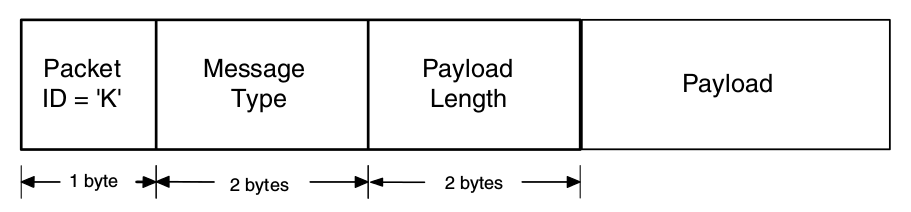
\includegraphics[scale=0.25]{gfx/signal_message}
\caption{Signal Nachricht (Quelle \cite{liang2006fasttrack})}
\label{fig:sigN}
\end{figure}

\subsection{Dem Netzwerk beitreten}
\label{subsec:join}

Der Ablauf, wenn sich ein Knoten in FastTrack Netzwerk verbindet ist in Abbildung \ref{fig:join} dargestellt.
Zuerst wählt der Knoten aus dem eigenen SN Cache ein paar SN.
Zu den gewählten SN wird eine \textit{UPD probe} Nachricht geschickt um zu testen ob der SN antworten, wenn dieser Antwortet wird ein TCP Handshake durchgeführt. 
Danach findet der Schlüsselaustausch statt, damit die folgenden Nachrichten verschlüsselt werden können.
Nun sendet der Knoten die Metadaten seiner Dateien zum SN und der SN eine Liste seiner bekannten SNs.
Mit dieser Liste aktualisiert der Knoten seinen SN Cache.
Wenn der SN Cache aktualisiert ist, bricht der Knoten die Verbindung ab und sucht sich aus der aktualisierte Listen einen Eltern SN. Die Möglichkeit der Wahl wird in \ref{subsubsec:wElternSN} beschrieben.
An diesem Eltern SN schickt seine Suchanfragen.

\begin{figure}
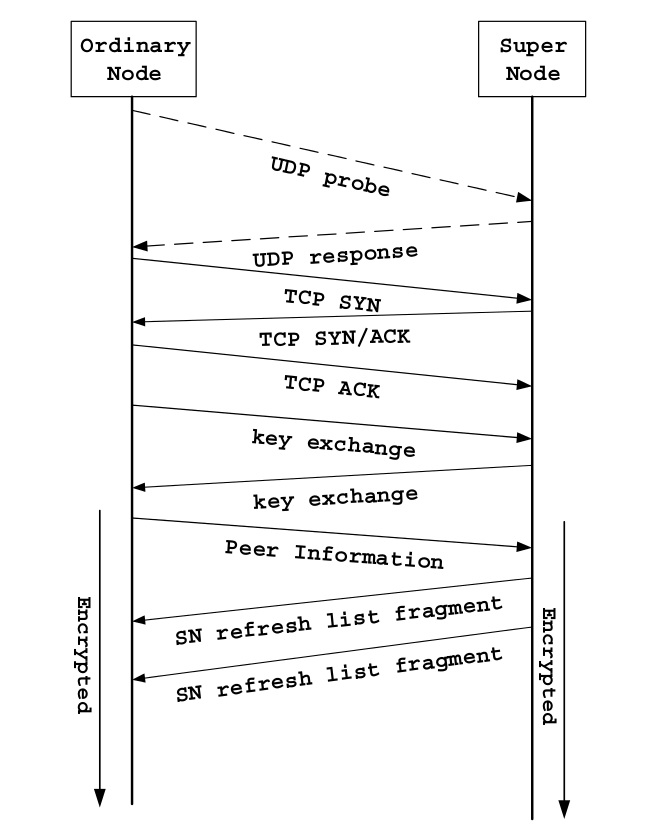
\includegraphics[scale=0.3]{gfx/join}
\caption{Nachrichten beim Verbindungsaufbau (Quelle \cite{liang2006fasttrack})}
\label{fig:join}
\end{figure}

\subsubsection{Wahl des Eltern SN}
\label{subsubsec:wElternSN}

Im Paper \cite{liang2006fasttrack} ist nicht genau bekannt nach welchen Kriterien der Eltern SN gewählt wird. 
Es werden zwei Möglichkeiten in Betracht gezogen.
Zum einen die Lokalität, das heißt wie weit der SN vom Knoten entfernt ist und zum anderen die Auslastung des SN.
Bei der Lokalität wird der RoundTripTime durch einen Ping zum SN gemessen.
In der Messung \ref{fig:rtt} ist zu erkennen, dass die meisten Knoten mit SN in ihrer Nähe verbunden sind.
Ein anderer Aspekt ist die Auslastung eines SN., diese wird mit im SN Cache des Knoten gespeichert.
Somit können beide Kriterien in die Wahl einbringen.

\begin{figure}
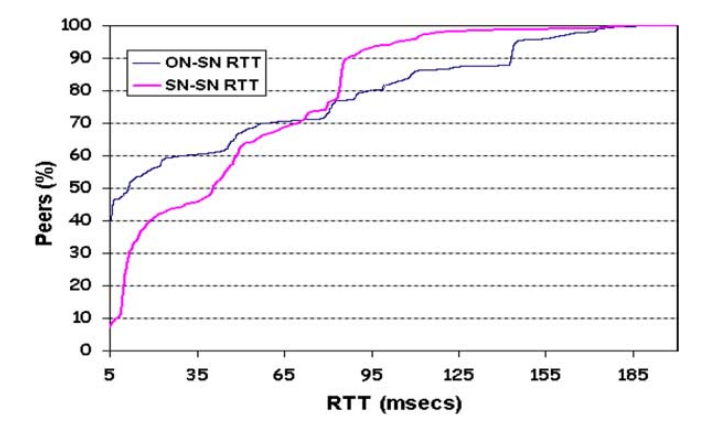
\includegraphics[scale=0.3]{gfx/rttSns}
\caption{RTT Knoten zu SN und SN zu SN (Quelle \cite{liang2006fasttrack})}
\label{fig:rtt}
\end{figure}

\subsection{Datenaustausch zwischen Superknoten}
\label{subsec:sntosn}

Der Ablauf wie die SNs untereinander ihre Daten austauschen ist in der Abbildung \ref{fig:snsn} dargestellt.
Wenn sich ein SN aktualisieren will, dann verbindet dieser sich zuerst über einen TCP Handshake mit dem SN aus seinem Cache um seine Liste oder Metadaten auszutauschen.
Nach dem TCP Handshake werden die Schlüssel austauscht.
Die folgenden Nachrichten der Metadaten und SN Listen werden nun verschlüsselt ausgetauscht.

\begin{figure}
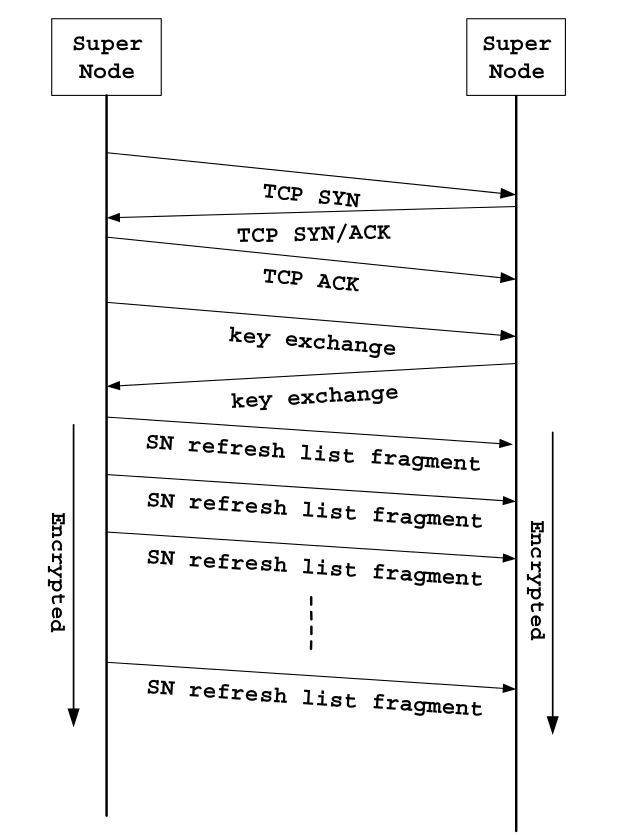
\includegraphics[scale=0.3]{gfx/SnToSn}
\caption{Nachrichten beim Austausch von Informationen zwischen SNs(Quelle \cite{liang2006fasttrack})}
\label{fig:snsn}
\end{figure}

\subsection{Suche im Netzwerk}
\label{subsec:search}

Wenn ein Knoten ein Datei suchen will, sendet dieser seinen Suchanfrage an seinen Eltern SN.
Dieser durchsucht die Metadaten seine bekannten Knoten und schickt die Antwort ob etwas gefunden wird zurück.
Außerdem wird die Suchanfrage an seine bekannte SN gesendet, damit dieser in den Metadaten seiner bekannten Knoten.
Mit der Antwort, kann der Knoten nun den Download starten.
In Sektion \ref{subsubsec:dnat} wird beschrieben wie der Download stattfindet, wenn der Knoten, welcher die Datei besitzt hinter eine Nat sitzt.

\subsubsection{Download über NAT}
\label{subsubsec:dnat}
Da es häufig vorkommt, dass die Knoten B hinter einem NAT sitzen, gibt es die Möglichkeit über den Eltern SN des jeweiligen Knoten, den Download zu starten.
Wenn ein Knoten A einen Download starten will, dann hat er die IP Adresse des Knoten B, daran erkennt er ob es eine lokale oder globale Adresse handelt.
Bei einer lokalen Adresse fragt er den Eltern SN des Knoten B, dass er von Knoten B eine Datei herunterladen will und nur die lokale Adresse kennt.
Der Eltern SN von B, teilt nun Knoten B mit, das Knoten A eine Datei von ihm herunterladen will.
Diese Nachricht enthält die globale Adresse von A.
Nun verbindet sich Knoten B mit Knoten A und Knoten A kann die Datei von B herunterladen.